\def\year{2018}\relax
%File: formatting-instruction.tex
\documentclass[letterpaper]{article} %DO NOT CHANGE THIS
\usepackage{aaai18}  %Required
\usepackage{times}  %Required
\usepackage{helvet}  %Required
\usepackage{courier}  %Required
\usepackage{url}  %Required
\usepackage{graphicx}  %Required
%\usepackage{times}
%\usepackage{graphicx}
\usepackage[caption=false]{subfig}
\usepackage{amsmath,amssymb}
\usepackage{algorithm,algorithmic}
\usepackage{color}
\usepackage{multirow}
\DeclareMathOperator*{\argmin}{argmin}
\hyphenation{Conv-Net}
%\newcommand{\xiaochuhao}{\fontsize{36pt}{\baselineskip}\selectfont}

\usepackage[american]{babel}

\frenchspacing  %Required
\setlength{\pdfpagewidth}{8.5in}  %Required
\setlength{\pdfpageheight}{11in}  %Required
%PDF Info Is Required:
  \pdfinfo{
/Title (Action Recognition with Coarse-to-Fine Deep Feature Integration and Asynchronous Fusion)
/Author (Weiyao Lin, Yang Mi, Jianxin Wu, Ke Lu, Hongkai Xiong)
}
\setcounter{secnumdepth}{2}





 \begin{document}
% The file aaai.sty is the style file for AAAI Press
% proceedings, working notes, and technical reports.
%
\title{Action Recognition with Coarse-to-Fine Deep Feature Integration and Asynchronous Fusion}
\author{Weiyao Lin$^1$\thanks{This work is supported in part by National Key Research and Development Program of China (2017YFB1002203), NSFC (61471235, 61571297, 61572316, 61720106001), Shanghai `The Belt and Road' Young Scholar Exchange Grant (17510740100), and Tencent research grant. Corresponding author is Weiyao Lin.}, Yang Mi$^1$, Jianxin Wu$^2$, Ke Lu$^3$, Hongkai Xiong$^1$\\
 $^1$ Department of Electronic Engineering, Shanghai Jiao Tong University, China\\
 $^2$ National Key Laboratory for Novel Software Technology, Nanjing University, China \\
 $^3$ University of Chinese Academy of Sciences, China \\
 \{wylin, deyangmiyang, xionghongkai\}@sjtu.edu.cn, wujx2001@nju.edu.cn, luk@ucas.ac.cn
 }

\maketitle

\begin{abstract}
  Action recognition is an important yet challenging task in computer vision. In this paper, we propose a novel deep-based framework for action recognition, which improves the recognition accuracy by: 1) deriving more precise features for representing actions, and 2) reducing the asynchrony between different information streams. We first introduce a coarse-to-fine network which extracts shared deep features at different action class granularities and progressively integrates them to obtain a more accurate feature representation for input actions. We further introduce an asynchronous fusion network. It fuses information from different streams by asynchronously integrating stream-wise features at different time points, hence better leveraging the complementary information in different streams. Experimental results on action recognition benchmarks demonstrate that our approach achieves the state-of-the-art performance.
\end{abstract}

\section{Introduction\label{section:introduction}}

Action recognition, which aims at identifying the action class label for an input action video, has attracted much attention due to its importance in many applications. Although the recent advances in deep convolutional networks (ConvNets) have brought some improvements on action recognition \cite{c3d,KVMF}, it remains challenging due to the large variation of video scenarios and the interferences from noisy contents unrelated to the video topic.

In this paper, we focus on two key issues for improving the performance over the existing ConvNet frameworks: (1) deriving more precise features to better represent actions, (2) reducing the asynchrony among information streams to better leverage the stream-wise complementary information.




%\begin{figure}[t]
%  \centering
%  \subfloat[]{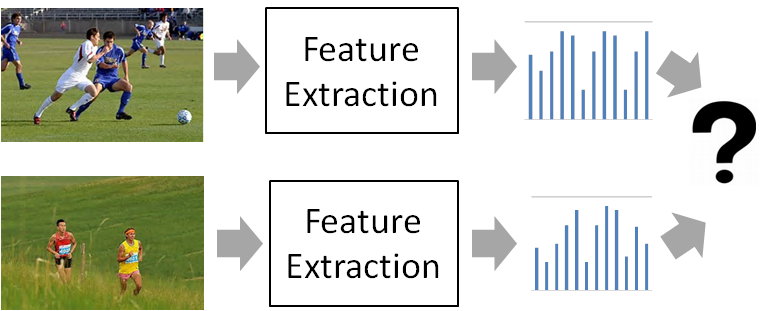
\includegraphics[width=3.6cm,height=1.3cm]{./figures1/fig1a.png}
 %   \label{fig:mapping structure_example_a}}\\
  %\hspace{3.2mm}
%  \subfloat[]{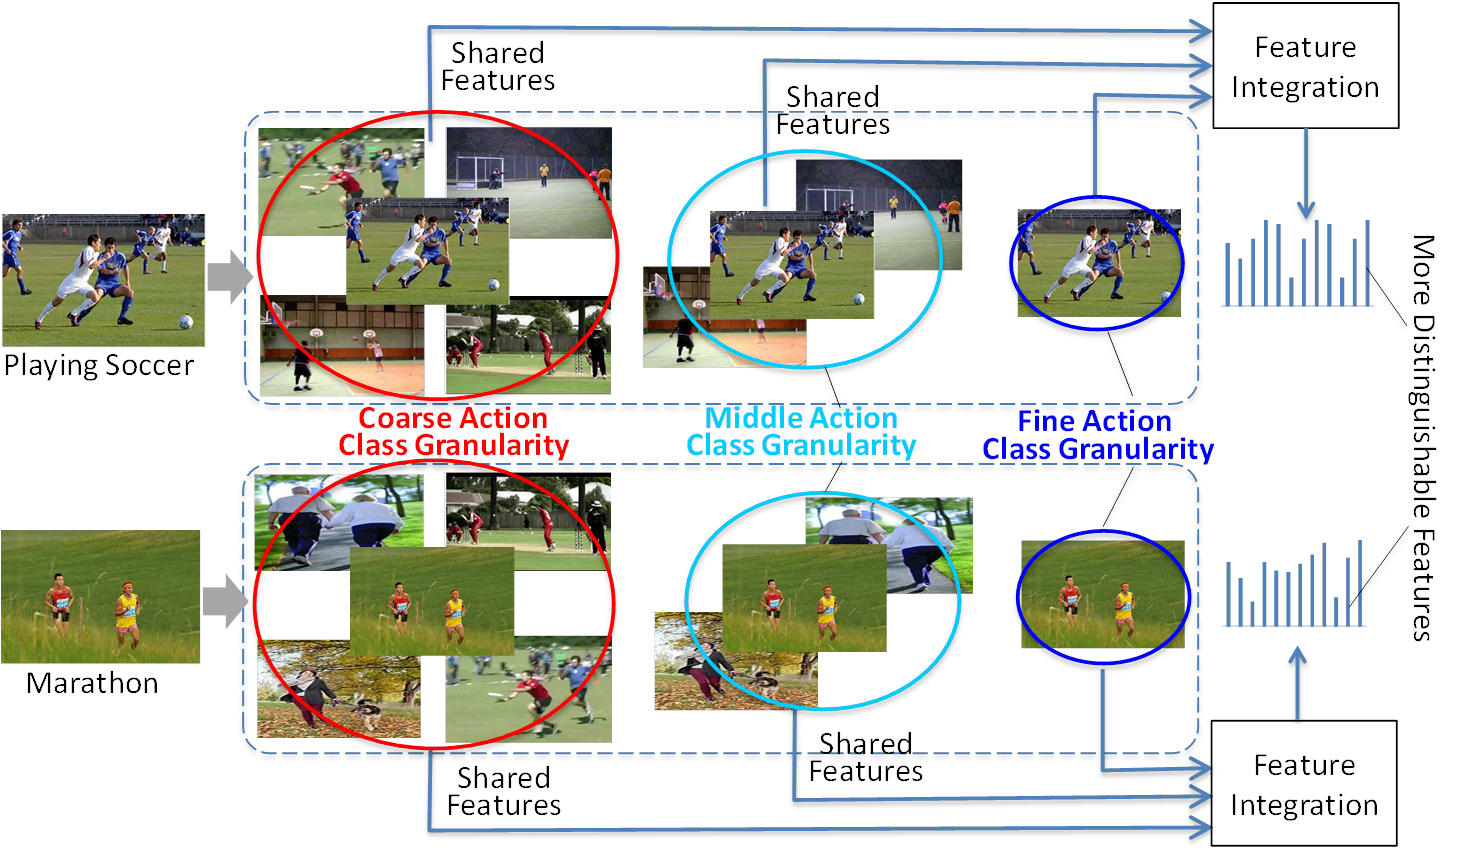
\includegraphics[width=8.0cm,height=4.8cm]{./figures1/fig1b.png}
%    \label{fig:mapping structure_example_b}}
 % \caption{Illustration of the idea of action class granularity. (a) When directly deriving features to recognize the individual action classes of visually similar video clips, it will be easily confused. (b)When deriving the shared features from action class groups with different granularities and integrate them together, the feature representation will
%  becombe more discriminative since the ambiguous action clips may correspond to different groups of action classes in coarser action class granularities. (Best viewed in color)}\label{fig:mapping structure_example}
%\end{figure}


%\begin{figure}
%  \centering
%  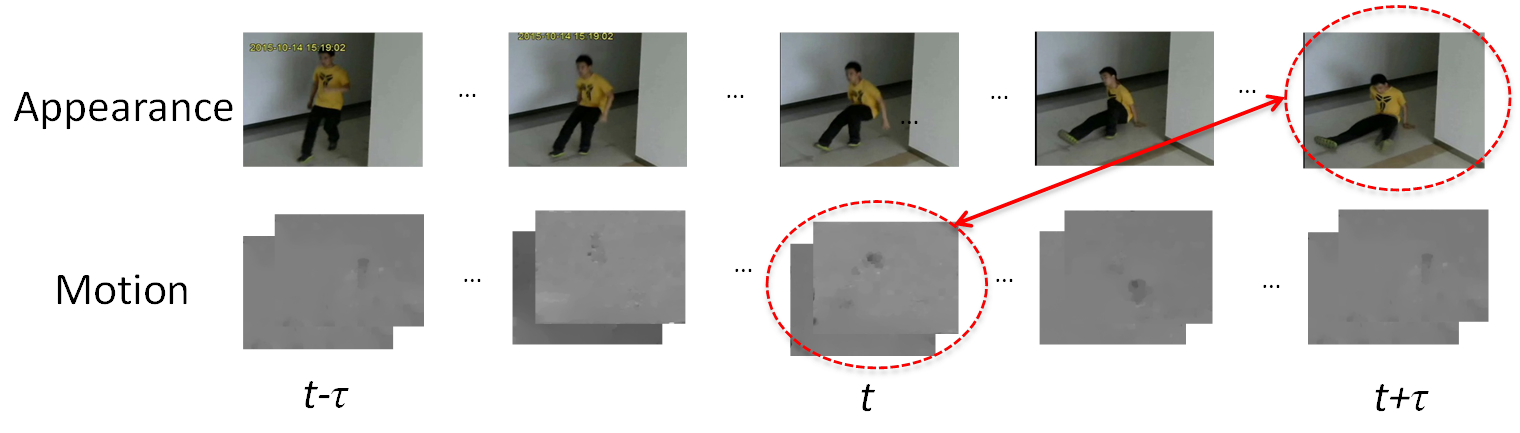
\includegraphics[width=0.475\textwidth]{./figures1/fig2.png}
%  \caption{An example of the asynchronous pattern between different information streams: The appearance stream shows the most indicative pattern about ``fall down" after the object has lied down on the floor, while the motion stream shows the strongest ``fall down" pattern when the object is in the process of going down.}
%    \label{fig:mapping structure_example_c}
%\end{figure}



First, good features are crucial to reliable action recognition. Although features automatically learned from ConvNets have shown big improvements in many domains~\cite{liu2016two,ImageNet,song2017end}, they make less progress in action recognition due to the high complexity of video data. Some recent studies attempted to improve the deep feature representation of an action by including additional information sources~\cite{dutaspatio,3stream,3stream2}, selecting spatial-temporal attention parts~\cite{kar2016adascan,visualattention,KVMF}, or incorporating more proper temporal information~\cite{TSN,cherian2017generalized}. However, since most of them focus on learning features to directly describe actions' individual action classes, they have limitations in precisely differentiating the ambiguity among action classes due to the large intra-class variations and subtle inter-class differences of actions.

\begin{figure}
  \centering
  %\subfloat[]{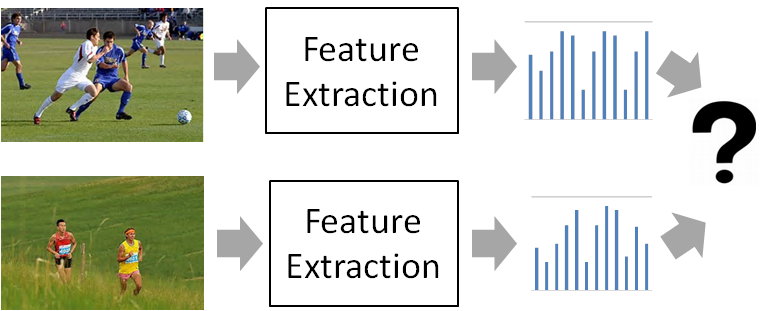
\includegraphics[width=3.6cm,height=1.3cm]{./figures1/fig1a.png}
  \subfloat[]{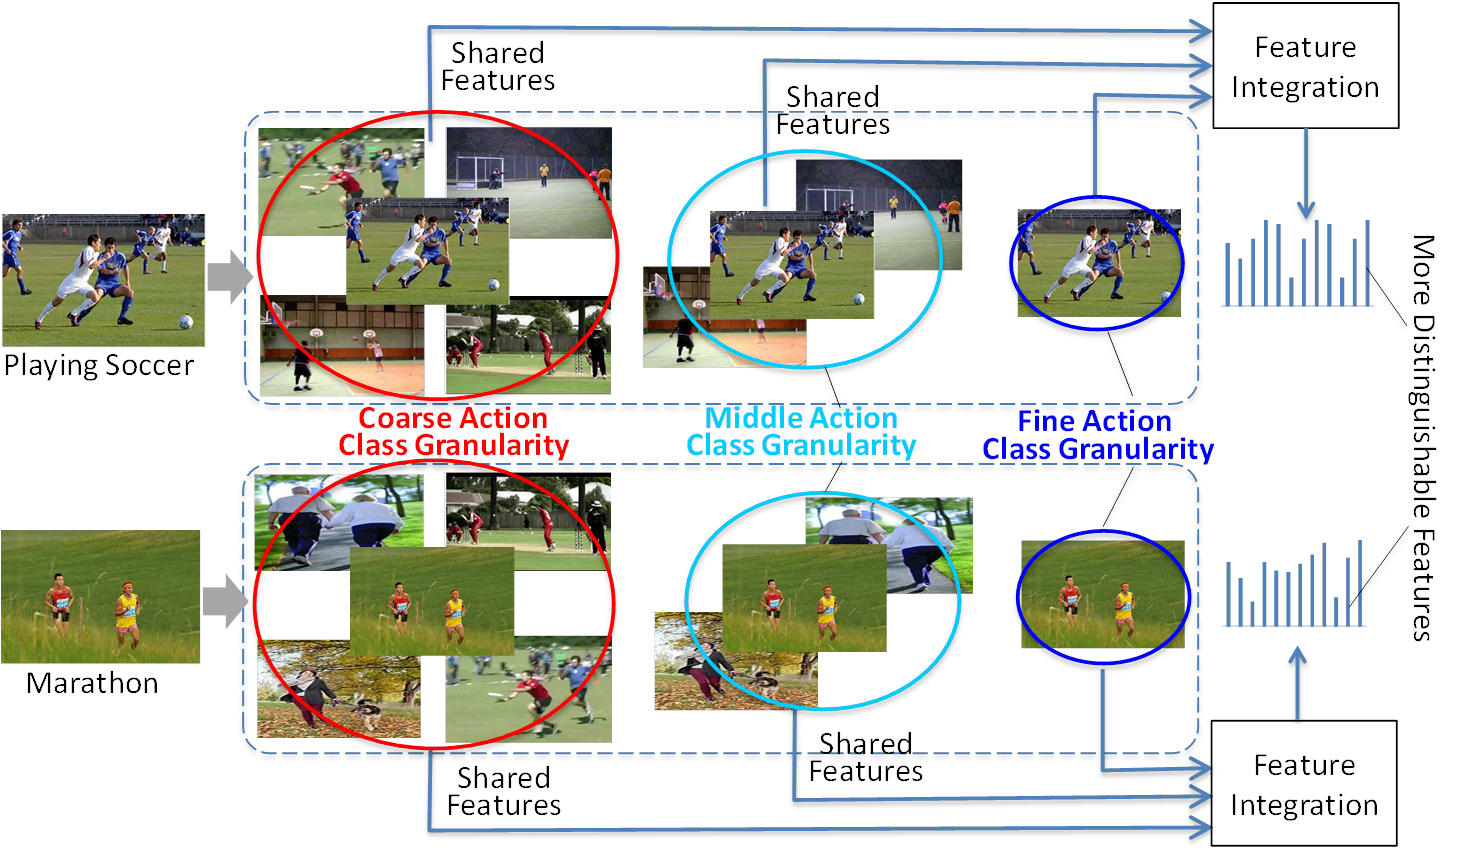
\includegraphics[width=8cm,height=4.5cm]{./figures1/fig1b.png} \label{fig:mapping structure_example_b}} \\
  %\vspace{-3.2mm}
  \subfloat[]{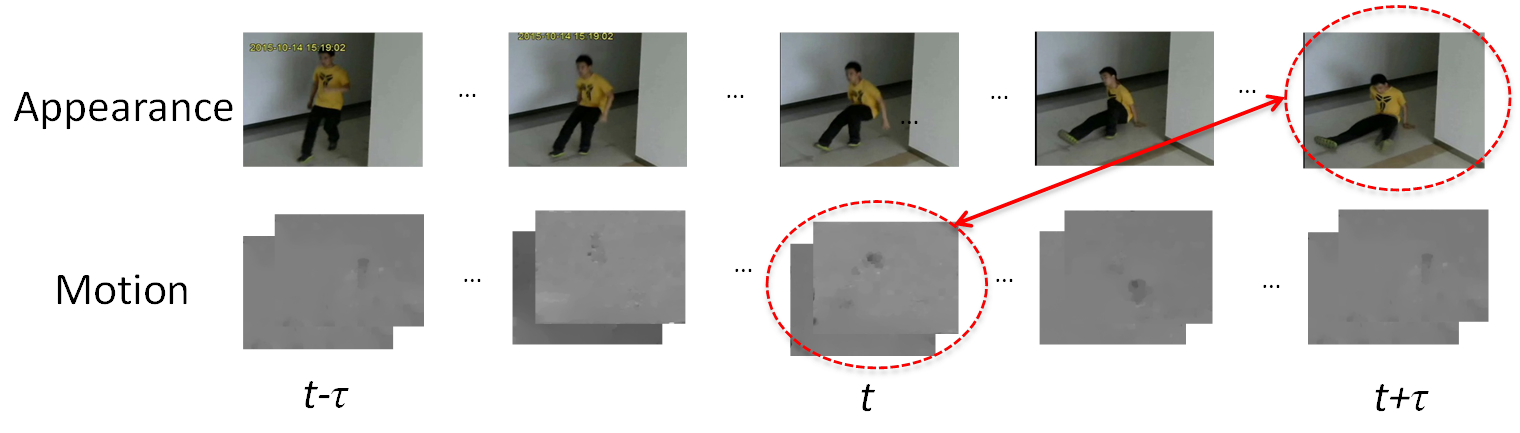
\includegraphics[width=0.45\textwidth,height=0.122\textwidth]{./figures1/fig2.png} \label{fig:mapping structure_example_c}}
  \caption{(a) Illustration of different action class granularity. (b) Illustration of the asynchronous pattern between streams: The appearance stream is most indicative about ``fall down" after the object has lied down, while the motion stream shows the strongest ``fall down" pattern when the object is in the process of going down. (Best viewed in color)} %When deriving the shared features from action class groups with different granularities and integrate them together, the feature representation will
%  becombe more discriminative since the ambiguous action clips may correspond to different groups of action classes in coarser action class granularities. (Best viewed in color)}
   % \label{fig:mapping structure_example_b}
\end{figure}

In this paper, we introduce the idea of \emph{action class granularity} where a coarser action class granularity includes more action classes and a finer action class granularity contains fewer action classes. We argue that features learned for different action class  granularities can provide useful information in discriminating action classes. For example, in Fig.~\ref{fig:mapping structure_example_b}, since the input action clip ``marathon" is visually similar to ``playing soccer", they will be easily confused if directly deriving features to recognize their individual action classes. However, if we relax the recognition requirement from individual action classes to action class groups (i.e., coarser action class granularities), we are able to obtain shared features for representing a set of action classes. These shared features are able to provide more discriminative power as ambiguous action clips may correspond to different groups of action classes in coarser action class granularities (cf. Fig.~\ref{fig:mapping structure_example_b}).

Based on this intuition, we propose a \emph{coarse-to-fine network} which first extracts deep features from different action class granularities, and then progressively integrates them from coarse granularities to fine ones to obtain a precise feature representation for input actions (cf. Fig.~\ref{fig:mapping structure_example_b}). It should be noted that since the action classes in each granularity are only used to derive proper features, they are automatically determined and dynamic for different input video clips.



Second, combining multiple information streams (such as two-stream ConvNets~\cite{baseline}) has shown strong performance and thus has become a mainstream framework in action recognition. However, most existing works only focus on introducing more information streams~\cite{3stream,3stream2} or strengthening the correlation among streams~\cite{TSN,wumultifusion,lstmiccv2017}, while the asynchronous issue among different information streams is less studied.

We argue that many actions have asynchronous patterns in different information streams, which affects the performance of action recognition. For example, Fig.~\ref{fig:mapping structure_example_c} shows two information streams for an action clip ``fall down" (one appearance stream and one motion stream). Apparently, the appearance stream shows the most indicative pattern about ``fall down" after the object has lied down on the floor. Comparatively, the motion stream shows the strongest ``fall down" pattern when the object is in the process of going down. If we simply combine the overall information in both streams or fuse the stream-wise information at the same time point, the indicative patterns appear at different time cannot be fully utilized and the performance is restrained. Therefore, we further introduce an \emph{asynchronous fusion network}, which asynchronously integrates stream-wise features from different time points, hence better leveraging the complementary information in multiple streams.

Overall, our contribution to action recognition are 3 folds:
\begin{enumerate}
 %\vspace{-8pt}
 \item We propose a coarse-to-fine network which extracts and integrates deep features from multiple action class granularities to obtain a more precise representation for actions.
 %\vspace{-8pt}
 \item We propose an asynchronous fusion network which integrates stream-wise features at different time points for better leveraging the information in multi-streams.
 %\vspace{-4pt}
 \item We combine the proposed coarse-to-fine and asynchronous fusion networks into an integrated framework which achieves the state-of-the-art performance.
\end{enumerate}

%\vspace{-4pt}
%The rest of this paper is organized as follows. Sec.~\ref{section:related_work} reviews related works. Sec.~\ref{section:overview} describes the overall framework of the proposed approach. Sections~\ref{section:Coarse-to-fine} and \ref{section:Asynchronuous} describe the details of our proposed coarse-to-fine and asynchronous fusion networks, respectively. Sec.~\ref{section:experimental evaluation} shows the experimental results and Sec.~\ref{section:conclusion} concludes the paper.


\section{Related Works\label{section:related_work}}

Action recognition has been studied for years. Early works focus on developing good hand-crafted features for representing actions, such as 3D SIFT~\cite{3dsift} and dense trajectory~\cite{iDT}. The performances for these methods are often restrained due to the limited differentiation capability of hand-crafted features.

With the development of deep ConvNets, many ConvNet-based methods were recently proposed for action recognition, which utilize ConvNets to automatically obtain the feature representation for actions. Ji et al.~\cite{3dcnn2} utilize a 3D ConvNet to recognize actions in video. Simonyan and Zisserman~\cite{baseline} propose a two-stream framework which uses two ConvNets to respectively extract features from two information streams (i.e., appearance and motion) and fuse them for recognition. Based on this framework, recent researches further improve the effectiveness of ConvNet features by including additional information sources~\cite{3stream,3stream2}, selecting spatial-temporal attention parts~\cite{kar2016adascan,visualattention,KVMF}, or incorporating more proper temporal information~\cite{TSN,wumultifusion,cherian2017generalized,DIN}.

Most of the existing works are targeted at learning features for directly describing actions' individual action classes, while the shared characteristics in different action class granularities are less studied. This restrains them from precisely distinguishing the subtle difference among ambiguous actions. Although some methods~\cite{jointattention} obtain different levels of generality by integrating features in multi-ConvNet layers, they still focus on directly representing the individual action classes and do not consider the shared characteristics in different action class granularities.

%Another thread of related works is the hierarchical classification techniques~\cite{hierarchical,hierarchical2} which gradually classify a sample from a larger class group to the final individual class. However, our approach differs from these methods in two aspects: (1) Hierarchical classification methods focus more on the progressive label classification of an input sample, which requires the class groups in each level to be pre-defined and fixed. Comparatively, our approach focuses on extracting the shared features from different action class granularities to improve the discriminativeness of features. The action classes in each granularity are only used to derive proper features, and thus are automatically determined and dynamic for different input action clips. (2) Most hierarchical classification methods need to manually construct multiple classifiers for different class groups. In contrast, our approach utilizes an integrated framework whose major components can be jointed constructed in an automatic way.

Besides the derivation of proper features, other researches focus on the proper combination of multiple information streams to boost the action recognition performance~\cite{nips,wumultifusion,twostreamfuse,lstmiccv2017}. For example, Feichtenhofer et al.~\cite{nips} introduce residual connections between information streams to remedy the deficiency of late fusion strategy in the two-stream framework. Wu et al.~\cite{wumultifusion} also improve the fusion efficiency of the two-stream framework by performing both sequence level fusion and video-level fusion over the information streams. However, most of these works fuse stream-wise information that happen simultaneously, which have limitations in handling the longer-term asynchronous pattern among information streams. As will be shown in this paper, the asynchrony among information streams is a non-trivial factor which can bring noticeable performance gains for action recognition.


\section{Overview}
\label{section:overview}

\begin{figure}
  \centering
  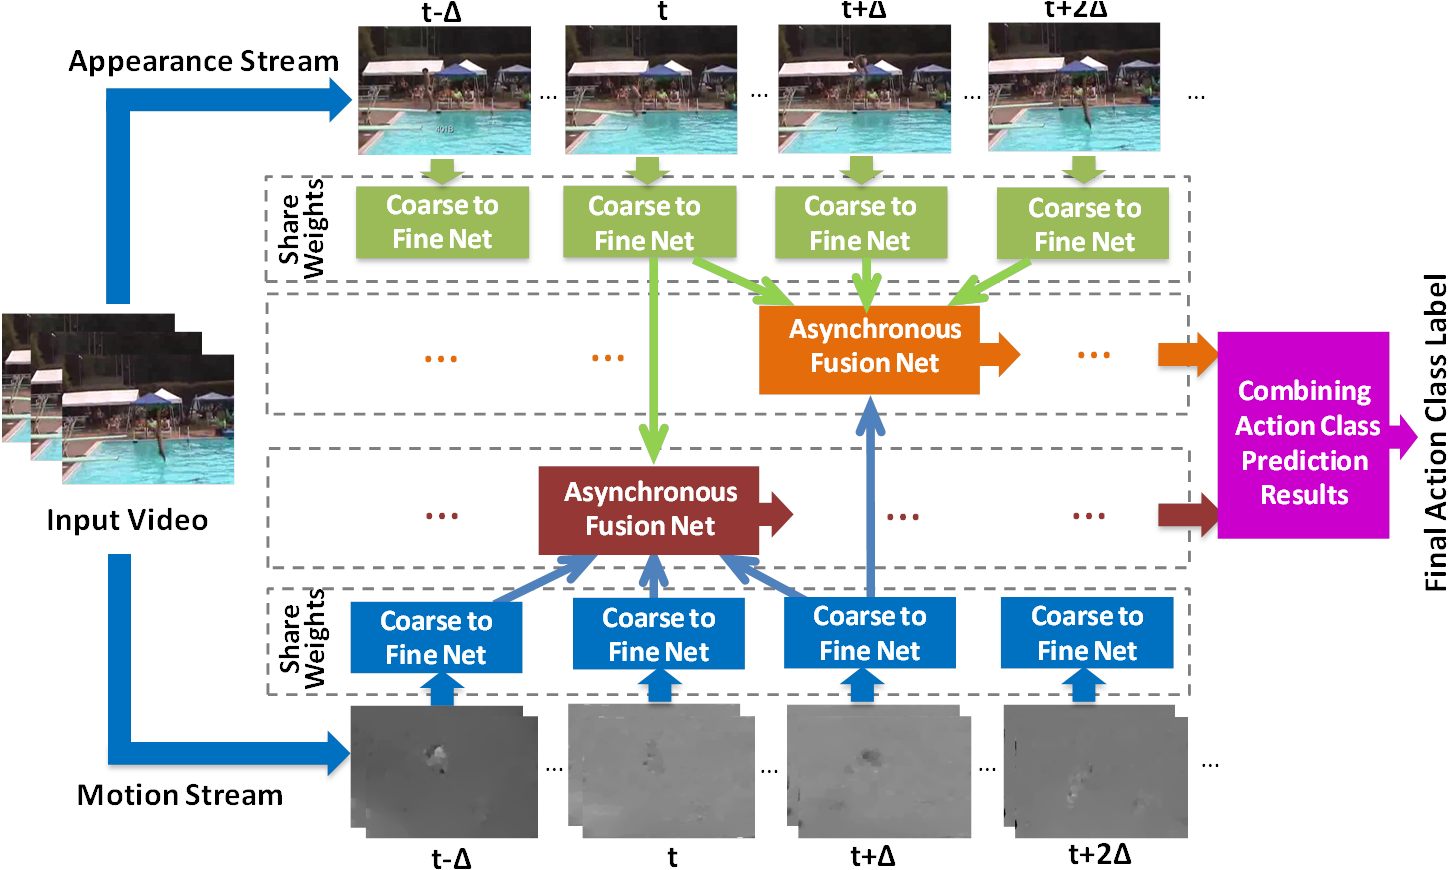
\includegraphics[width=0.47\textwidth,height=0.30\textwidth]{./figures1/framework.png}
  \caption{Framework of the approach. The coarse-to-fine network (detailed in Fig.~\ref{fig:coarse-to-fine}) extracts a more precise feature representation for each frame/optical flow stack. These features are then fused by asynchronous fusion networks (detailed in Fig.~\ref{fig:asynchronous}) to obtain action prediction results.}
    \label{fig:framework}
\end{figure}

The framework of our approach is shown in Fig.~\ref{fig:framework}. After obtaining appearance and motion streams from an input video, we first input each spatial frame from the appearance stream and each short-term optical flow stack from the motion stream into a coarse-to-fine network (detailed in Sec.~\ref{section:Coarse-to-fine}), which integrates deep features from multiple action class granularities and creates a more precise feature representation. The extracted features are then fed into asynchronous fusion networks (detailed in Sec.~\ref{section:Asynchronuous}), where each asynchronous fusion network integrates stream-wise features at different time points within a period and obtains an action class prediction result. Finally, action prediction results from different asynchronous fusion networks are combined to decide the final action class of the input video.

Note that the framework of our approach is integrated where the major components in the coarse-to-fine and asynchronous fusion networks can be jointly trained.%{\footnote {Source code for our approach will be released later.}} %, as detailed in Sec.~\ref{section:Asynchronuous}.

%end-to-end trainable where the coarse-to-fine and asynchronous fusion networks can be jointly trained and constructed. Since the coarse-to-fine network and the asynchronous fusion network are the key contributions of our approach, we describe the  details of them in Sections~\ref{section:Coarse-to-fine} and \ref{section:Asynchronuous}, respectively.




%Based on this intuition, we propose a coarse-to-fine process which first extracts shared deep features from multiple action class groups, and then integrates them to obtain a precise feature representation for an input action. In order to make the feature more precisely capture the pattern of the input action, we further introduce a class-ranking net to automatically construct action class groups with different granularities (i.e., action class groups with different numbers of action classes, as the red-circled groups in Fig.~\ref{fig:mapping structure_example_b}), and utilize a Recurrent Neural Network (RNN) model to progressively integrate the shared features from coarse-grain action class groups to fine-grain ones.



\section{Coarse-to-Fine Network\label{section:Coarse-to-fine}}



The structure of the coarse-to-fine network is shown in Fig.~\ref{fig:coarse-to-fine}. Basically, the network includes three major modules: first, a \emph{multi-granularity feature extraction} module is applied over a ConvNet to extract deep features from different action class granularities. Second, in order to guarantee the extraction of proper features in the feature extraction module, an \emph{adaptive class group forming} module is introduced. This module adaptively forms a suitable action class group for each action class granularity of an input frame/optical flow stack, so as to guide the feature extraction module to create the desired features. Third, a \emph{coarse-to-fine integration} module is connected to the feature extraction module, which progressively integrates features from coarse action class granularities to fine ones and outputs a precise feature representation for the input frame/optical flow stack.

It should be noted that the \emph{adaptive class group forming} module is only used in the training stage, while the \emph{multi-granularity feature extraction} and \emph{coarse-to-fine integration} modules are applied in both training and testing stages.


%In this section, we introduce the concept of coarse to fine network, showing the structure of coarse to fine network and the scheme of shared feature extraction and finally fuse the coarse to fine features to perform frame level prediction. We use static image for spatial stream and optical flow for temporal stream. The paper mainly demonstrate the spatial stream and the same structure can be constructed for temporal stream.

\begin{figure}
  \centering
  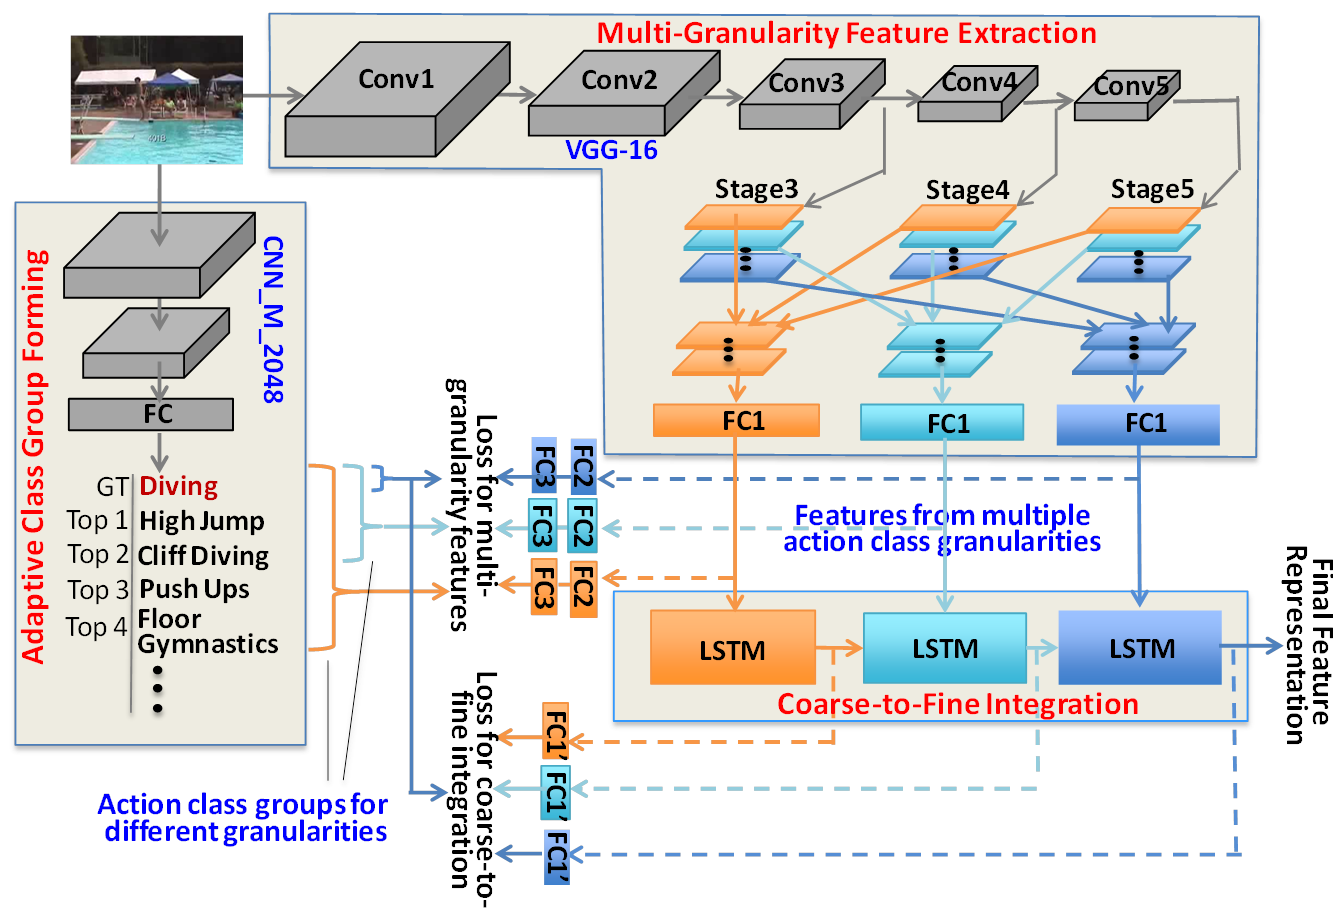
\includegraphics[width=0.47\textwidth,height=0.32\textwidth]{./figures1/coarse-to-fine.png}
  \caption{Structure of the coarse-to-fine network.}
    \label{fig:coarse-to-fine}
\end{figure}


\subsection{Multi-granularity feature extraction}

%\subsection{Aliasing structure of multi-scale feature}

The multi-granularity feature extraction module aims to extract deep features from different action class granularities. Since side output layers have shown their effectiveness in encoding multi-scale information in skeleton \& boundary detection~\cite{skeleton,skeleton2}, we borrow them into action recognition and construct three side output flows to extract features in three action class granularities.

Specifically, we derive side output maps from the last convolutional layer in stages $3$, $4$, and $5$ of VGG-$16$ ConvNet (i.e., conv3\_3, conv4\_3, conv5\_3). The side output maps from different stages are then sliced and concatenated into three scale-specific side map groups~\cite{skeleton}, where each side map group corresponds to one action class granularity. In order to ensure output maps from different stages to have the same size, upsampling layers are applied on side output maps before map concatenating. Finally, the scale-specific side map groups are input into a fully connected (FC) layer respectively to obtain features for the three action class granularities (FC$1$ in  Fig.~\ref{fig:coarse-to-fine}). Note that different from the previous side output works~\cite{skeleton,skeleton2}, our approach utilizes an FC layer in the side output flow  to obtain features for describing actions.


%As mentioned,our network contains multi-level fineness and multi-scale features to model different action category group. Recent work []demonstrate fine-tuning on pre-trained neural network architecture can be very helpful to obtain good performance on a new task. We basically adopt the VGG-16 network architecture[] as the fundamental feature extraction pipeline and add additional side output streams for different category group convergence at different deep layers. We connect the proposed scale-associated side output stream to the last three convolutional layer in each stage except for the first two stage, respectively,conv3\_3,conv4\_3,conv5\_3. The receptive field sizes of the scale-associated side output streams are 40, 92, and 196, respectively. Each side output stream are then provided with certain number of similar action categories. With category group produced by ranking net, each side stream can extract corresponding shared features for certain action group. In order to make each scale-associated stream consider more comprehensive information, we use the slicing and concatenation for the fundamental feature maps, and then the different upsampling kernel size for different scale, such that each side stream not only extract features at different scale, but also different action group. An illustration for the network architecture is shown in Fig.4.



%As mentioned, action categories may share various features including objects, static scenes and movements, leading to small inter-class distance, which makes direct prediction of final label difficult. Thus, we introduce the coarse to fine network to get the final prediction progressively. Firstly, we extract feature maps from different layers of CNN network and get shared features of multi-scale, as shown in fig3. These shared feature contains abundant multi-scale categories and across-categories information, which are very helpful for group and precise action label prediction. Then we use LSTM net to fuse shared features of different scales, thus the coarse to fine network can produce a more discriminative feature for action recognition. Within the whole process, several points need to be mentioned about the net.(1)While extracting coarse representation, we combine features of different deep layers, such that each scale feature can contain more comprehensive information.(2) in order to obtain reasonable shared feature of similar action group at different scale, we introduce a category ranking net and utilize its group label output to constrain the training process of this network, as shown in dashed box of fig.2.(Note that, this framework is only used for training).(3)we utilize LSTM for multi-scale shared feature fusion, for the reason that, our coarse to fine framework produce features of category group with different similarity, which forms a sequence of coarse to fine features, and LSTM network can properly and progressively encode the sequence features, that helps a lot.



\subsection{Adaptive class group forming}

The \emph{adaptive class group forming} module is a key part of the coarse-to-fine network, which aims to form suitable action class groups to guide the feature extraction process in the \emph{multi-granularity feature extraction} module. In this paper, we introduce an additional smaller ConvNet (i.e., CNN\_M\_$2048$~\cite{M2048}) to form action class groups in different granularities.

Specifically, we first use the CNN\_M\_$2048$ ConvNet to predict the action class label of an input frame/optical flow stack, and then use the top $5$, top $3$, and top $1$ action classes in the predicted result to form the action class groups in the three action class granularities, respectively.

Three important issues need to be mentioned about the \emph{adaptive class group forming} module: (1) The \emph{adaptive class group forming} module is only applied in the training stage which helps to construct a reliable multi-granularity feature extracion network. During the testing stage, the feature extraction module will directly output features without the guidance of action class groups. (2) The CNN\_M\_$2048$ ConvNet is pre-trained on the same dataset and is fixed during the training process. We fix the CNN\_M\_$2048$ ConvNet in training in order to create stable action class groups. (3) When forming action class groups, if the groundtruth label of an input frame/optical flow stack is not listed in the top ranked action group in CNN\_M\_$2048$'s prediction result, we will mandatorily include it into the action class group to avoid the feature extraction module deriving irrelevant features to the input frame/optical flow stack.

After action class groups are constructed in the \emph{adaptive class group forming} module, they are used to guide the feature extraction process by a cross-entropy loss~\cite{crossentropy}, which forces the feature extraction module to create shared features that best describe the constructed action class groups in multiple granularities:

\begin{equation}
\begin{aligned}
\mathcal{L}_v(\mathbf{W})=&-\frac{1}{N}\sum_{k=1}^{3}\sum_{n\in \mathbf{G}_k}{{\alpha }_{k}\log{\hat{p}(n|\mathbf{W},k)}}\\
\end{aligned}
\label{equation:equ0}
\end{equation}
where $\mathbf{W}$ is the parameter set for the \emph{multi-granularity feature extraction} module. $N$ is the total number of action classes. $\mathbf{G}_k$ is the constructed action class group for the $k$th action class granularity and ${\alpha }_{k}$ is the weight measuring the relative importance of the $k$th action class granularity. $\hat{p}(n|\mathbf{W},k)$ is the probability for the $n$th action class predicted by the features from $k$th action class granularity. Note that in order to create action prediction results $\hat{p}(n|\mathbf{W},k)$, two additional fully connected layers are added to the feature output layer of the \emph{multi-granularity feature extraction} module in the training stage (FC$2$ \& FC$3$ in Fig.~\ref{fig:coarse-to-fine}).


\begin{figure}
  \centering
  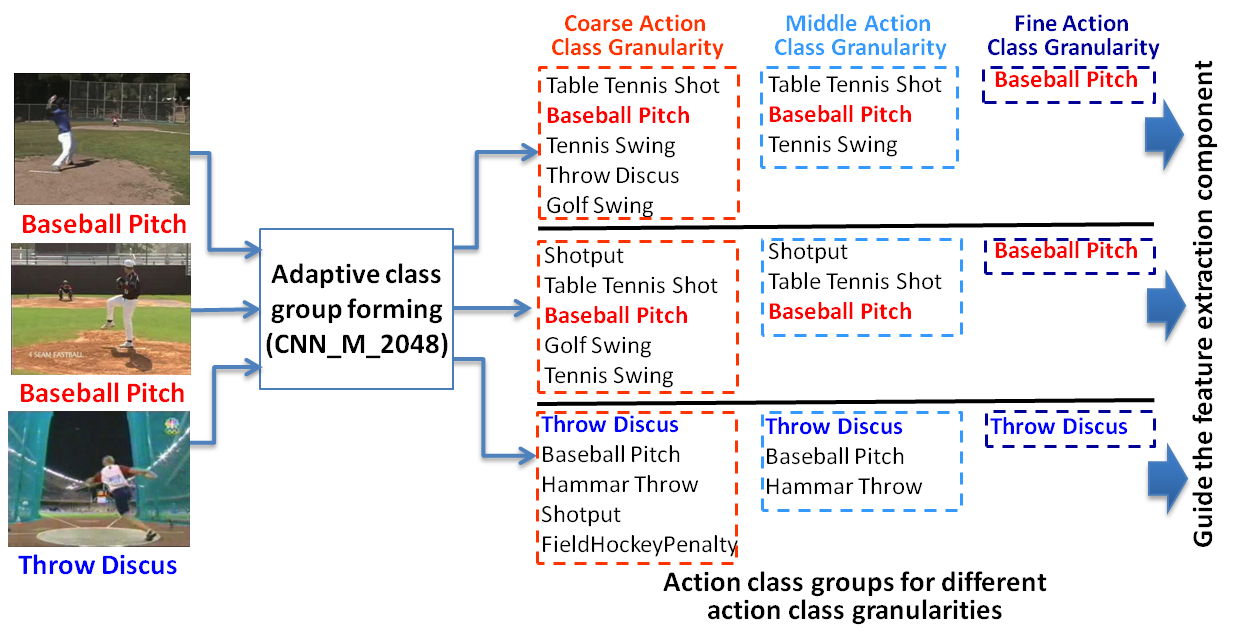
\includegraphics[width=0.47\textwidth,height=0.28\textwidth]{./figures1/action_class.png}
  \caption{Examples of the adaptively formed action class groups for different inputs (best viewed in color).}
    \label{fig:action-class}
\end{figure}

We argue that by introducing the CNN\_M\_$2048$ ConvNet to form action class groups, we can have three advantages:

\begin{enumerate}
 %\vspace{-8pt}
 \item Since the CNN\_M\_$2048$ ConvNet is pre-trained on the same dataset, it has the capability to properly parse the action class contents of an input frame/optical flow stack. Thus, it is able to create informative action class groups which are relatively more similar for same-class inputs and less similar for different-class inputs (cf. the action class groups for the two ``Baseball Pitching" inputs and the ``Throw Discus" input in Fig.~\ref{fig:action-class}). Therefore, when using these action class groups to guide the feature extraction process, we are able to obtain more distinguishable features. Note that the CNN\_M\_$2048$ ConvNet does not need to be perfectly trained. From our experiments, CNN\_M\_$2048$  roughly trained from partial data is already able to create good results (cf. Sec.~\ref{Datasets_experimental settings}).
     %For example, in Fig.~\ref{fig:action-class}, two {\color{red}``Baseball Pitching"} inputs have more similar action class groups, while another easily confusable input {\color{red}``Throw Discus"} creates less similar the action class groups.
 %\vspace{-8pt}
 \item Since the ground-truth action class of an input frame/optical flow stack is included in each of its action class groups (cf. the red and blue bold action classes in Fig.~\ref{fig:action-class}), features guided by these action class groups are able to capture the characteristics of the input's true action class in different aspects. Therefore, by integrating features from multiple action class granularities (cf. Sec.~\ref{integration}), the feature representation is properly strengthened, which has stronger capability to predict the correct action class for the input sample. %Note that this is an important point which guarantees to obtain reliable performances even if the action class groups do not

 %\vspace{-4pt}
 \item Moreover, by introducing CNN\_M\_$2048$ ConvNet into our coarse-to-fine network, we are also taking the advantage of properly combining two ConvNets (i.e., CNN\_M\_$2048$ and VGG-$16$) to boost action recognition performances. As will be shown in the experimental results, our approach provides a more proper way to combine ConvNets, which has obviously better performance than only using a single ConvNet or combining ConvNets in simpler ways~\cite{twocnn,twocnn2}.

%\item construct a more reasonable ConvNet for modeling the characteristics of actions. Specifically, a video may include many \emph{noisy} frames/optical flow stacks whose appearance/motion characteristics are confusing and less related to its groundtruth action label. If we only use the groundtruth label to guide the training process of a ConvNet, the ConvNet may be misled and result in an improper model. For example, in Fig. 1 (b) in the paper, the frame at $t-\tau$ looks more like ``walking'' and is less related to the groundtruth label ``falling down''. If forcibly using label ''falling down'' in training, the ConvNet model maybe misled and misclassify some true ''walking'' images as ``falling down''. However, if we use multi-grain action labels, a more reasonable ConvNet model can be obtained. In the above example, our approach can use a coarse label set including both ``walking'' and ``falling down'' to guide the training of ConvNet. In this way, the constructed ConvNet can not only capture the information cues for the groundtruth label ``falling down'', but also construct a reasonable correlation between ``walking'' and its appearance characteristics. Thus, the chance of misclassifying true ``walking'' images is properly reduced.
\end{enumerate}

%Shared features of certain action group is the key part of our framework and this part corresponds to two aspects. Firstly, we need a method to search the similar categories for static frame or optical flow volume and second use these grouped category information to constrain the training process such to get reasonable shared feature for recognition. In principle, any clustering methods can be used for action group division. However, due to the enormous difference of deep neural network and common clustering methods like kMeans, these methods cannot find proper deep similar categories. In our work, we use a short and rough recognition neural network, which is based on CNN\_M\_2048, and fix its parameters during the training of coarse to fine network. Compared with VGG\_16, this architecture contains less deep layers and the larger convolutional kernels and is pretrained with samples of small size. The recognition accuracy of this ranking net is about 0.2, a very rough recognition and thus this ranking net can find more similar categories for the frame and optical flow volume input. Following the CNN\_M\_2048 net, we sort its output possibility for each action class, and chose the top K class labels as the label group for each shared feature stream, with progressively smaller K to help each side stream extract multi precision shared features, shown as Figure 1. Note that if top K don not contains ground truth label of image or optical flow volume, we add the original label into top K labels, forming K+1 label group, such that each side stream will not diverge from the correct prediction. After obtaining the label group, we use the multi-label loss function(XXX) for the side stream to converge to label group rather than single label. Though these group label converge, we can extract shared features of frame or optical flow volume which can represent a group of similar action categories. These shared features are of great significance for final recognition.

\subsection{Coarse-to-fine integration}\label{integration}

After obtaining features from multiple action class granularities, we further utilize a \emph{coarse-to-fine integration} module to progressively integrates features from different action class granularities and outputs a precise feature representation. In this paper, we utilize a Long Short Term Memory (LSTM) network to perform coarse-to-fine integration due to its effectiveness in fusing sequential inputs~\cite{LSTM,LSTM2}.

%The input and output relation for an LSTM unit is shown by:

%\begin{equation}
%\begin{aligned}
%\mathbf{i}_{t} &= \sigma \left ( \mathbf{M}_{xi}\mathbf{x}_{t}+ \mathbf{M}_{hi}\mathbf{h}_{t-1}+\mathbf{b}_{i}\right)
%\\\mathbf{f}_{t}&= \sigma \left ( \mathbf{M}_{xf}\mathbf{x}_{t}+ \mathbf{M}_{hf}\mathbf{h}_{t-1}+\mathbf{b}_{f}\right)
%\\\mathbf{c}_{t}&= \mathbf{f}_{t}\odot \mathbf{c}_{t-1}+\mathbf{i}_{t}\odot \tanh \left ( \mathbf{M}_{xc}\mathbf{x}_{t}+ \mathbf{M}_{hc}\mathbf{h}_{t-1}+\mathbf{b}_{c}\right)
%\\\mathbf{o}_{t}&= \sigma \left ( \mathbf{M}_{xo}\mathbf{x}_{t}+ %\mathbf{M}_{ho}\mathbf{h}_{t-1}+\mathbf{b}_{o}\right)
%\\\mathbf{g}_{t} &= \tanh \left ( \mathbf{M}_{xc}\mathbf{x}_{t}+ \mathbf{M}_{hc}\mathbf{h}_{t-1}+\mathbf{b}_{c}\right)
%\\\mathbf{h}_{t}&= \mathbf{o}_{t}\odot \tanh\left ( \mathbf{c}_{t} \right )
%\end{aligned}
%\label{equation:equ1}
%\end{equation}
%where $\mathbf{i}_{t}$, $\mathbf{f}_{t}$, and $\mathbf{o}_{t}$ represent the input gate, forget gate, and output gate, respectively~\cite{LSTM,LSTM2}. $\mathbf{c}_{t}$ is the unit state. $\mathbf{h}_{t-1}$ is the hidden state results from the previous unit. $\mathbf{x}_{t}$ is the current feature input. $\sigma$ is sigmoid function and $\odot$ is element-wise product operator. $\mathbf{M}$ and $\mathbf{b}$ are LSTM unit parameters.

Specifically, we utilize an LSTM model with three units, where each unit takes features $\mathbf{x}_{t}$ from one action class granularity and creates hidden state outputs $\mathbf{h}_{t}$ to influence the next unit (cf. Fig.~\ref{fig:coarse-to-fine}). The hidden state output from the last unit will be the final integrated feature for the input frame/optical flow stack. The entire process is described by: %Eq.~\ref{equation:equ2}.

\begin{equation}
\begin{aligned}
\mathbf{h}_{1}&={F}_{\mathbf{\Phi}_1}\left ( \mathbf{x}_{1}, 0 \right )
\\\mathbf{h}_{2}&={F}_{\mathbf{\Phi}_2}\left ( \mathbf{x}_{2},\mathbf{h}_{1} \right )
\\\mathbf{h}_{3}&={F}_{\mathbf{\Phi}_3}\left ( \mathbf{x}_{3},\mathbf{h}_{2} \right )
\end{aligned}
\label{equation:equ2}
\end{equation}
where $\mathbf{x}_{t}$ and $\mathbf{h}_{t}$ ($t=1,2,3$) are the input features and hidden state results for $t$th LSTM unit. $\mathbf{\Phi}_t=\{\mathbf{M}_t, \mathbf{b}_t\}$ is the parameter set for $t$th unit and ${F}_{\mathbf{\Phi}_t}$ is the operation of $t$th unit to create hidden state outputs~\cite{LSTM}.  %as in Eq.~\ref{equation:equ1}.

In the training stage, we utilize the following loss function to train LSTM model to create the desired results.

\begin{equation}
\begin{aligned}
\mathcal{L}_l(&\mathbf{\Phi}_1,\mathbf{\Phi}_2,\mathbf{\Phi}_3)=-\frac{\beta}{N} ( \log{\hat{p}(n_g|\mathbf{\Phi}_1)}\\&+
\log{\hat{p}(n_g|\mathbf{\Phi}_1,\mathbf{\Phi}_2)}+\log{\hat{p}(n_g|\mathbf{\Phi}_1,\mathbf{\Phi}_2,\mathbf{\Phi}_3)}  )
%\sum_{t=1}^{3}{{\beta }_{t}\log{\hat{p}(n_g|\mathbf{\Phi}_t)}}\\
\end{aligned}
\label{equation:equ3}
\end{equation}
where $\mathbf{\Phi}_1,\mathbf{\Phi}_2,\mathbf{\Phi}_3$ are the parameter sets for the three units in LSTM. $\beta$ is the weight measuring the relative importance of the LSTM model. $n_g$ is the ground-truth action class label for an input sample. $N$ is the total number of action classes. $\hat{p}(n_g|\mathbf{\Phi}_1..\mathbf{\Phi}_t)$ is the predicted probability for the ground-truth class from the $t$th unit. Similar to Eq.~\ref{equation:equ0}, in order to create action prediction probability $\hat{p}(n_g|\mathbf{\Phi}_1..\mathbf{\Phi}_t)$, an additional fully connected layer is added to the output of each LSTM unit in the training stage (cf. FC$1'$ in Fig.~\ref{fig:coarse-to-fine}).


%\begin{equation}
%\begin{aligned}
%\left(
%  \begin{array}{c}
 %         \mathbf{i}_{t} \\
%          \mathbf{f}_{t} \\
%          \mathbf{o}_{t} \\
%%          \mathbf{g}_{t}
% \end{array}
% \right)&=   \left(
 % \begin{array}{c}
%          \sigma \\
 %         \sigma \\
 %         \sigma \\
 %         \tanh
% \end{array}
%  \right)\left(\mathbf{\Phi}
%    \left(
 %   \begin{array}{c}
%          \mathbf{h}_{t-1} \\
%          \mathbf{x}_{t} \\
% \end{array}
% \right)+\left(
% \begin{array}{c}
 %{b}_{i}\\
% {b}_{f}\\
% {b}_{o}\\
% {b}_{c}
%  \end{array}
% \right)
% \right)\\
%{i}_{t} = \sigma \left ( {W}_{xi}{x}_{t}+ {W}_{hi}{h}_{t-1}+{b}_{i}\right)
%\\f_{t} = \sigma \left ( {W}_{xf}{x}_{t}+ {W}_{hf}{h}_{t-1}+{b}_{f}\right)
%\\o_{t} = \sigma \left ( {W}_{xo}{x}_{t}+ {W}_{ho}{h}_{t-1}+{b}_{o}\right)
%\\g_{t} = \tanh \left ( {W}_{xc}{x}_{t}+ {W}_{hc}{h}_{t-1}+{b}_{c}\right)
%\begin{center}
%\mathbf{c}_{t} &= \mathbf{f}_{t}\odot \mathbf{c}_{t-1}+\mathbf{i}_{t}\odot \mathbf{g}_{t}\\
%\mathbf{h}_{t} &= \mathbf{o}_{t}\odot \tanh\left ( \mathbf{c}_{t} \right )
%\end{center}
%\end{aligned}
%\label{equation:equ1}
%\end{equation}


\subsection{Loss function for coarse-to-fine network}

The loss function for the coarse-to-fine network is shown by: %in Eq.~\ref{equation:equ44}.

\begin{equation}
\begin{aligned}
\mathcal{L}_{\mathcal{C}}(\mathbf{\Psi}_{\mathcal{C}})=\mathcal{L}_v(\mathbf{W})+\mathcal{L}_l(\mathbf{\Phi}_1,\mathbf{\Phi}_2,\mathbf{\Phi}_3)%+{\gamma}(\sum {{w}^{2}}+\sum{{\phi}^{2}})
\end{aligned}
\label{equation:equ44}
\end{equation}
where $\mathcal{L}_v(\mathbf{W})$ and $\mathcal{L}_l(\mathbf{\Phi}_1,\mathbf{\Phi}_2,\mathbf{\Phi}_3)$ are the losses for the \emph{multi-granularity feature extraction} and \emph{coarse-to-fine integration} modules, respectively. $\mathbf{\Psi_{\mathcal{C}}}=\{\mathbf{W},\mathbf{\Phi}_1,\mathbf{\Phi}_2,\mathbf{\Phi}_3\}$ is the parameter set for the entire coarse-to-fine network.%$\sum {{w}^{2}}+\sum{{\phi}^{2}}$ ($w\in\mathbf{W},{{\phi}\in\{\mathbf{\Phi}_1,\mathbf{\Phi}_2,\mathbf{\Phi}_3\}}$) is the term measuring model complexity~\cite{LSTMSRC}, and $\gamma$ is the balancing weight.

Note that the coarse-to-fine network can be jointly trained with the asynchronous fusion network in our approach. Therefore, Eq.~\ref{equation:equ44} can be further combined with the loss of the asynchronous fusion network to construct a final loss function for the entire approach, as will be discussed in Sec.~\ref{section:Asynchronuous}.




%entire coarse to fine network consists of four parts, fundamental feature extraction pipeline, additional side streams, LSTM fusion network and ranking net. For side streams and LSTM fusion network, a good loss function plays an important role for the whole network. In order each part and the entire coarse to fine network can converge to reasonable parameters, we introduce cross-entropy loss for label group coupled with multinomial logistic loss for single label to constrain the training process . The loss function is defined as  (\ref{equation:equ3}):
%\begin{equation}
%\begin{aligned}
%E=&\frac{-1}{N}\sum_{k=1}^{2}\sum_{n=1}^{N}{\gamma }_{k}({p}_{kn}\log {\hat{p}_{kn}}+(1-{p}_{kn})\log(1- {\hat{p}_{kn}}))
%\\&+\frac{-1}{N}{\gamma }_{3}\sum_{n=1}^{N}\log {\hat{p}_{n,{l}_{n}}}+\frac{-1}{N}{\gamma }_{lstm}\sum_{t=1}^{3}\sum_{n=1}^{N}{p}_{kn}\log {\hat{p}_{kn}}
%\\&+{\gamma}_{\theta}\sum\sum {\theta}_{i,j}^{2}\\
%\end{aligned}
%\label{equation:equ3}
%\end{equation}
%Where k is the stage of side streams, p is the one hot label vector,  $\hat{p}$ is the output class probabilities, $\gamma$ is the loss weight coefficient for each part, and  $\theta$ represents all the model parameters. Demonstrated by the experiments, without loss function item for each stage of shared feature extraction, the former stage will be overwhelmed by the final stage feature extraction, which is harmful for shared feature extraction and action recognition.

\section{Asynchronous Fusion Network}\label{section:Asynchronuous}

The structure of the asynchronous fusion network is shown in Fig.~\ref{fig:asynchronous}. Basically, the asynchronous fusion network aims to fuse an input feature at time $t$ in one stream with multiple input features around $t$ in another stream, so as to leverage the stream-wise complementary information at different time points. It mainly includes two modules: First, the \emph{stream-wise feature fusion} module is used to fuse two input features from different streams. Second, the \emph{asynchronous integration} module is used to integrate the fused outputs over different time and create an action class prediction result for the period of the input features.

\begin{figure}
  \centering
  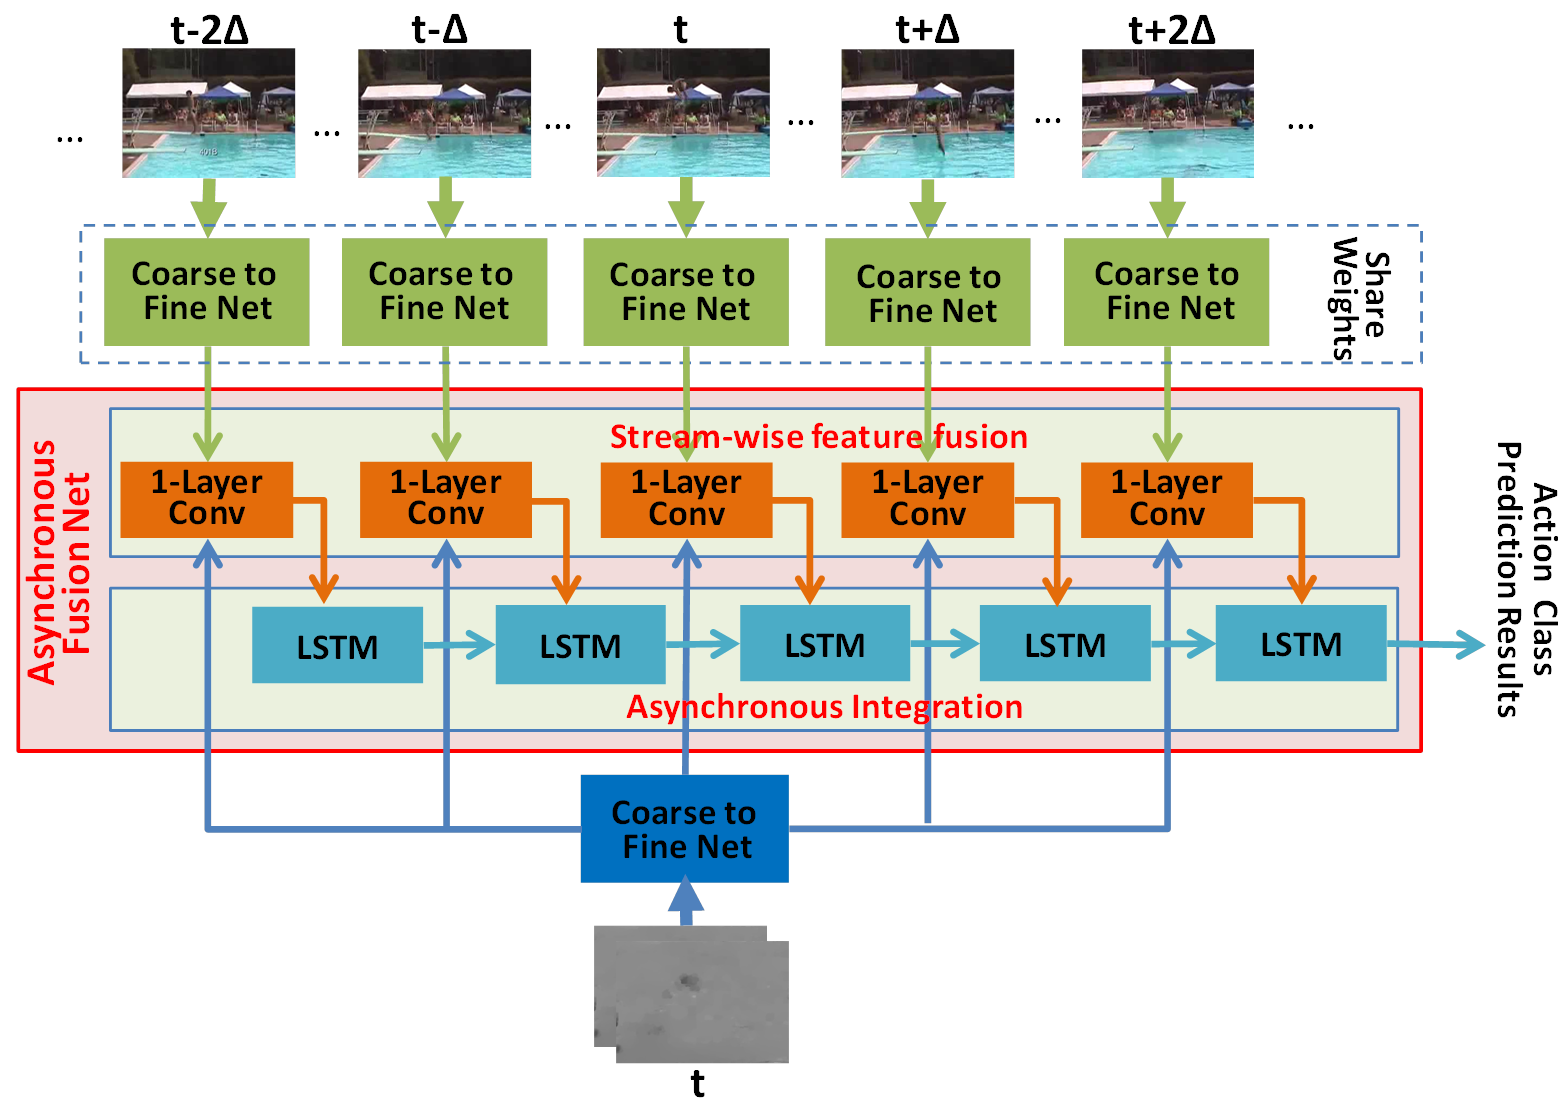
\includegraphics[width=0.43\textwidth,height=0.27\textwidth]{./figures1/asynchronous.png}
  \caption{Structure of asynchronous fusion network and its relation with coarse-to-fine networks.} %(Note that the structure can also be used to fuse one frame input and multiple optical flow stack inputs. Best viewed in color)}
    \label{fig:asynchronous}
\end{figure}


\subsection{Stream-wise feature fusion}

Since inputs from different information streams have different characteristics, simply concatenating them may create less effective fusion results. Therefore, we utilize a ConvNet to fuse features from different streams due to its effectiveness in fusing multi-stream inputs~\cite{twostreamfuse}. Since input features are only $1$-dimensional vectors, we simply view them as two $1$-dimensional feature maps and apply a single layer ConvNet with $1\times 1$ kernel to create the fused output.


Note that: (1) In our asynchronous fusion network, an input feature in one stream is fused with $5$ input features from another stream. Therefore, five $1$-layer ConvNets are used to fuse stream-wise features (cf. Fig.~\ref{fig:asynchronous}). (2) Moreover, the five input features to be fused also have $\Delta$ ($\Delta=5$) time intervals to each other. This enables us to capture the longer-term asynchronous patterns between streams.



%Since input features from each stream are one dimensional, the cascaded features are two dimensional. Therefore, the kernel sizes of $3$D CNNs in our approach are actually simplified into $m\times m\times 1$.


\subsection{Asynchronous integration}

After obtaining stream-wise fusion results with different time intervals, the \emph{asynchronous integration} module will sequentially integrate them and create an action prediction result for the period of the input features. In this paper, we utilize a five-unit LSTM to perform integration (cf. Fig.~\ref{fig:asynchronous}) since it has good capability in integrating sequential inputs~\cite{LSTM}. %The structure of LSTM and input-output relation for each LSTM unit is the same as Sec.~\ref{integration}.


\subsection{Loss function for the asynchronous fusion network \& the entire framework}

The entire asynchronous fusion network can be trained by:

\begin{equation}
\begin{aligned}
\mathcal{L}_{\mathcal{A}}(\mathbf{\Psi}_\mathcal{A})=-\frac{\gamma}{N} \sum_{t=1}^{T}\log{\hat{p}(n_g|\mathbf{\Phi}_1,..,\mathbf{\Phi}_t,\mathbf{K}_1,..,\mathbf{K}_t)}
%\\&+
%{\beta }_{2}\log{\hat{p}(n_g|\mathbf{\Phi}_1,\mathbf{\Phi}_2)}+{\beta }_{3}\log{\hat{p}(n_g|\mathbf{\Phi}_1,\mathbf{\Phi}_2,\mathbf{\Phi}_3)}  )
%\sum_{t=1}^{3}{{\beta }_{t}\log{\hat{p}(n_g|\mathbf{\Phi}_t)}}\\
\end{aligned}
\label{equation:equ5}
\end{equation}
where $N$ is the total number of action classes. $n_g$ is the ground-truth class label of input video. $T=5$ is the total number of LSTM units and $1$-layer ConvNets. $\mathbf{\Phi}_t$ and $\mathbf{K}_t$ are the parameter sets for the $t$th LSTM unit and $t$th $1$-layer ConvNet, respectively. $\mathbf{\Psi_{\mathcal{A}}}=\{\mathbf{\Phi}_1,...,\mathbf{\Phi}_T,\mathbf{K}_1,...,\mathbf{K}_T\}$ and $\gamma$ are the parameter set and weight for the entire asynchronous fusion network, respectively. $\hat{p}(n_g|\mathbf{\Phi}_1,...,\mathbf{\Phi}_t,\mathbf{K}_1,...,\mathbf{K}_t)$ is the predicted probability for the ground-truth class from the $t$th LSTM unit.


%$$ is the predicted probability for the ground-truth class from the $t$th unit.

Moreover, the asynchronous fusion network can be jointly trained with the coarse-to-fine network by combining their loss functions. Therefore, the overall framework of our approach can be trained by:


\begin{equation}
\begin{aligned}
(&\mathbf{\Psi}_{\mathcal{C},s_1},\mathbf{\Psi}_{\mathcal{C},s_2},\mathbf{\Psi}_{\mathcal{A}})^*= \\ &\mathop{\argmin}{(\sum_{t=1}^T{\mathcal{L}_{\mathcal{C}}^{t}(\mathbf{\Psi}_{\mathcal{C},s_1}})}+  \mathcal{L}_{\mathcal{C}}(\mathbf{\Psi}_{\mathcal{C},s_2})+\mathcal{L}_{\mathcal{A}}(\mathbf{\Psi}_\mathcal{A}))
\end{aligned}
\label{equation:equ6}
\end{equation}
where $\mathbf{\Psi}_{\mathcal{C},s_1}$, $\mathbf{\Psi}_{\mathcal{C},s_2}$ are the parameter sets of the coarse-to-fine networks for the first and second information streams. $\mathbf{\Psi}_{\mathcal{A}}$ is the parameter set of the asynchronous fusion network. $\mathcal{L}_{\mathcal{C}}(\cdot)$ and $\mathcal{L}_{\mathcal{A}}(\cdot)$ are the loss functions of the coarse-to-fine and asynchronous fusion networks (cf. Eqs.~\ref{equation:equ44} and \ref{equation:equ5}). $T=5$ is the total number of inputs in the first stream (cf. Fig.~\ref{fig:asynchronous}). Note that since the five coarse-to-fine networks in the first stream share weights, we use the same parameter set $\mathbf{\Psi}_{\mathcal{C},s_1}$ to calculate the loss of each input $\mathcal{L}_{\mathcal{C}}^{t}(\mathbf{\Psi}_{\mathcal{C},s_1}), t=1,...,5$.

Besides, it should also be noted that our approach actually requires to construct two independent models, where one model fuses an appearance-stream input with multiple motion-stream inputs, and another model fuses a motion-stream input with multiple appearance-stream inputs. The action prediction results from both models and at different time periods are then combined to decide the final label of an input video (cf. Fig.~\ref{fig:framework}). In this paper, we follow the mainstream two-stream methods~\cite{TSN} to combine action prediction results, which adds the action prediction results from different models \& periods and selects the class with the largest overall prediction score as the final result.



\section{Experimental Results\label{section:experimental evaluation}}

\subsection{Datasets \& experimental settings}\label{Datasets_experimental settings}

{\bf Datasets.} We perform experiments on two benchmark datasets: UCF$101$~\cite{ucf101} and HMDB$51$~\cite{hmdb51}. UCF$101$ dataset is a commonly used dataset for action recognition. It contains $13,320$ video clips in $101$ action classes. HMDB$51$ dataset is a large collection of realistic videos, which contains $6,766$ video clips in $51$ action classes.

%Our experiments follow the original evaluation scheme using three training/testing splits and report average accuracy over these splits.

{\bf Experimental settings.} We implement our approach on Caffe~\cite{caffe}. The batch size and momentum are set to be $16$ and $0.9$, respectively. The weight parameters for different granularities in the coarse-to-fine network ($\alpha_1,\alpha_2,\alpha_3$ in Eq.~\ref{equation:equ0}) are set to be $0.1$, $0.1$, $1$ respectively. Besides, the weight parameters for the LSTM models in the coarse-to-fine and asynchronous fusion networks ($\beta$ and $\gamma$ in Eqs.~\ref{equation:equ3} and \ref{equation:equ5}) are set as $2$ to let the networks focus more on the reliability on their final outputs.


We use the same method as~\cite{TSN,TDDIDT,transform} to construct optical flow stacks and perform data augmentation. Moreover, the VGG-16 models in both appearance and motion streams are initialized with a pre-trained model from ImageNet~\cite{ImageNet}. When training the entire framework, we set the initial learning rate as $10^{-2}$ and is decreased to its $1/10$ for every $20$K iterations. The maximum iteration is $100$K. Besides, the CNN\_M\_$2048$ ConvNet used to construct action class groups are trained with $1/8$ of the training data and $10$K iterations.

During evaluation, we sample $12$ periods from each video, where each period includes $5$ frames and $5$ corresponding optical flow stacks with temporal distance $\Delta=5$ (cf. Fig.~\ref{fig:asynchronous}). The prediction results from these periods are combined to obtain the final result.





%We use the popular publicly available CNN toolbox Caffe and use the mini-batch stochastic gradient descent algorithm to learn the network parameters.In the training process ,we set batch size to 16 and momentum to 0.9. For the coarse to fine network, we initialize it with the pre-trained models from ImageNet[Deng, J., Dong, W., Socher, R., Li, L., Li, K., Li, F.: ImageNet: A large-scale hierarchical image database. In: CVPR. (2009) 248{255] and the loss weight for the first, second stage is 0.1, the third stage is 1 and the loss weight for LSTM shared feature fusion is 2 for the reason that we use loss for every stage to converge and mainly focus on the final LSTM output shared features. For the part of asynchronous network, we set the loss weight for each stage 0.2 and the LSTM fusion loss weight to 1, which constrain the entire network to converge more regularly.We set a similar learning rate in our experiments. The initial learning rate is 0.001 and decreases to 0.0001 after 30K iteration, 0.00001 after 50K iteration, 0.00001 after 80K iteration and stops at the 130K iteration. As for data augmentation, we use the techniques of randomly cropping, flipping, mirroring and rotating, which is helpful for avoiding overfitting. For optical flow extraction, we use the Brox[T. Brox, A. Bruhn, N. Papenberg, and J. Weickert. High accuracy optical flow estimation based on a theory for warping. In Proc. ECCV, pages 2004.] algorithm implemented in OpenCV with CUDA.

\subsection{Results for the coarse-to-fine network}\label{section:results for coarse to fine}

In order to evaluate the effectiveness of our coarse-to-fine network, we compare six methods: (1) The standard two-stream approach~\cite{baseline} ({\emph{Two-stream baseline}}). (2) Combining $2$ two-stream networks (VGG-$16$ and CNN\_M\_$2048$) by fusing their fully connected layers for recognition~\cite{twocnn,twocnn2} ({\emph{Direct combine ConvNets}}). (3) Delete the {\emph{adaptive class group forming} module and only use the loss function in Eq.~\ref{equation:equ3} to train the coarse-to-fine network ({\emph{CO2FI-no class grouping}}). (4) Delete the coarsest action class granularity and only use the two finer action class granularities in our coarse-to-fine network for recognition ({\emph{CO2FI-two granularities}}). (5) Use three action class granularities in the coarse-to-fine network, but each granularity only contains a single ground-truth action class ({\emph{CO2FI-no coarseness}}). (6) The complete version of our coarse-to-fine network ({\emph{CO2FI-complete}}). %(6) Roughly pre-train CNN\_M\_$2048$ ConvNet with $1/8$ of the training data and $10$K iterations, and use it to form action class groups in our coarse-to-fine network ({\bf\emph{CO2FI-rough class grouping}}). (7) The complete version of our coarse-to-fine network ({\bf\emph{CO2FI-complete}}).

%\renewcommand{\multirowsetup}{\centering}
\begin{table}
\centering
\caption{Results of coarse-to-fine network (split1)}\label{tab:cmcTable1}
\scriptsize{
\label{table1}
\begin{tabular}{|p{0.85cm}|c|*{5}{c|}c}
\hline
{}&\textbf{Methods}& Appearance& Motion& 2-stream \\
\hline
\multirow{6}*{{\tiny{\bf{UCF101}}}}
&Two-stream baseline& {79.2\%}& {84.8\%}& {89.8\%} \\
&Direct combine ConvNets& {80.1\%}& {85.4\%}& {90.6\%} \\
&CO2FI-no class grouping& {79.1\%}& {85.2\%}& {90.0\%} \\
&CO2FI-two granularities& 81.0\%& 86.9\%& 91.7\% \\
&CO2FI-no coarseness& 79.5\%& 85.4\%& 90.4\% \\
&{\bf CO2FI-complete}& {\bf 81.7\%}& {\bf 87.9\%}& {\bf 92.8\%}  \\
\hline
\multirow{2}*{{\tiny{\bf{HMDB51}}}}
&Two-stream baseline& {48.1\%}& {55.4\%}& {58.4\%} \\
&{\bf CO2FI-complete}& {\bf 55.5\%}& {\bf 63.0\%}& {\bf 67.9\%}  \\
\hline
\end{tabular}}
\end{table}

Table~\ref{tab:cmcTable1} compares the action recognition results on split $1$ of UCF$101$ and HMDB$51$ datasets, where the mean classification accuracy for appearance stream, motion stream, and two-streams are listed. Note that in order to delete the effect of the asynchronous fusion network in this experiment, we directly add a softmax layer after the coarse-to-fine network to obtain recognition results. From Table~\ref{tab:cmcTable1}, we can observe:

(1) The performance of the \emph{CO2FI-no class grouping} method is similar to \emph{two-stream baseline} and is obviously lower than the complete version of our approach (\emph{CO2FI-complete}). This implies that without the guidance of the \emph{adaptive class group forming} module, the coarse-to-fine network will construct less precise features and bring few improvements. Besides, the $\emph{Direct combine ConvNets}$ method also achieves less obvious improvements. This further indicates that satisfactory results cannot be easily obtained without a proper way to combine ConvNets.

(2) Comparing the \emph{CO2FI-no coarseness} method with the \emph{CO2FI-two granularities} method, we can see that less noticeable improvements are obtained if each action class granularity only contains one ground-truth action class (\emph{CO2FI-no coarseness}). Comparatively, when each action class granularity includes more action classes, more obvious improvements are achieved with only two action class granularities (\emph{CO2FI-two granularities}). This indicates that the shared characteristics from multiple action classes are the key parts to improve feature representations, and the improvements are restrained if these shared characteristics cannot be obtained (as in \emph{CO2FI-no coarseness}).

(3) The complete version of our coarse-to-fine network (\emph{CO2FI-complete}), which obtains features by including more action class granularities with different coarseness, has the largest improvement over the baseline. This further demonstrates the effectiveness of our approach.

%Comparing the \emph{CO2FI-complete} method with the \emph{CO2FI-two granularities} method, we can see that a higher recognition result can be achieved in \emph{CO2FI-complete} by introducing an additional action class granularity.



%Comparing \emph{CO2FI-rough class grouping} method with \emph{CO2FI-complete} method, we can see that satisfactory performances can be achieved when only using a roughly trained CNN\_M\_$2048$ ConvNet (\emph{CO2FI-rough class grouping}) to form action class groups in our coarse-to-fine network. This demonstrates the flexibility of our approach. Moreover, the performances are further improved when a more finely tuned CNN\_M\_$2048$ ConvNet is included for forming action class groups (\emph{CO2FI-complete}).

%Moreover, the last two rows in Table~\ref{tab:cmcTable1} also show the performance of our coarse-to-fine network on HMDB$51$ dataset, which also shows that the proposed coarse-to-fine network can also obtain obvious improvements over the baseline.


\subsection{Results for the asynchronous fusion network}

Table~\ref{tab:cmcTable2} shows the performance of our asynchronous fusion network. In Table~\ref{tab:cmcTable2}, the upper part shows the results by applying the fusion network on the baseline two-stream ConvNet (i.e., \emph{Baseline+SYN}, \emph{Baseline+ASYN}), and the lower part shows the results by combining our fusion network with the coarse-to-fine network (\emph{CO2FI+ASYN}). Moreover, \emph{SYN} refers to the method that fuses two stream-wise features at the same time point. \emph{ASYN ($\Delta=1$)} and \emph{ASYN ($\Delta=5$)} mean using our asynchronous fusion network to fuse stream-wise features, where the temporal distances of input features being fused are $1$ and $5$ (cf. Fig.~\ref{fig:asynchronous}).



\begin{table}
\centering
\caption{Results of asynchronous fusion network (split 1) %(note: the \emph{appearance} results of \emph{ASYN-Fusion} refer to the results by fusing one appearance input feature with multiple motion input features)
}\label{tab:cmcTable2}
\scriptsize{
%\label{table2}
\begin{tabular}{|p{4.5cm}|c|*{5}{c|}c}
\hline
\textbf{Methods}& UCF101& HMDB51 \\
\hline
Two-stream baseline &  89.8\%& 58.4\% \\%\\
Baseline+SYN & 89.7\%& --\\
Baseline+ASYN ($\Delta=1$) & 90.3\% & -- \\
{\bf Baseline+ASYN ($\Delta=5$)}&  {\bf 91.0\%} &{\bf 60.9\%}\\
\hline
%CO2FI (rough)+ASYN & 93.2\%& 68.3\%  \\
CO2FI & 92.8\%& 67.9\%  \\
{\bf CO2FI+ASYN ($\Delta=5$)}& {\bf 93.7\%}& {\bf 69.5\%}  \\
\hline
\end{tabular}}
\end{table}


%Specifically, \emph{SYN-Fusion} refers to the method that fuses two stream-wise features at the same time point and combines their action prediction results over time. \emph{ASYN-Fusion ($\Delta=1$)} and \emph{ASYN-Fusion ($\Delta=5$)} mean using our asynchronous fusion network to fuse stream-wise features, where the temporal distances of features being fused are $1$ and $5$, respectively (cf. Fig.~\ref{fig:asynchronous}). %Note that for \emph{ASYN-Fusion} methods, the \emph{appearance} and \emph{motion} results in Table~\ref{tab:cmcTable2} refer to the results by fusing one appearance stream input with multiple motion stream inputs, and fusing one motion stream input with multiple appearance stream inputs, respectively.

From the upper part of Table~\ref{tab:cmcTable2}, we can see that simply fusing features at the same time point brings no improvements (\emph{Baseline+SYN}). When we only fuse stream-wise features that are temporally close to each other (\emph{Baseline+ASYN ($\Delta=1$)}), the improvements are still less obvious since the longer-term asynchronous patterns are not properly captured. Comparatively, when fusing stream-wise features with larger temporal distances (\emph{Baseline+ASYN ($\Delta=5$)}), we can obtain more noticeable improvements. This demonstrates that the asynchrony between different information streams indeed affects action recognition performances. Moreover, from the lower part of Table~\ref{tab:cmcTable2}, we can also observe that when combining our asynchronous fusion network with the coarse-to-fine network, we can obtain further improved recognition performances by leveraging both mutli-granularity features and stream-wise complementary information (\emph{CO2FI+ASYN ($\Delta=5$)}).

Fig.~\ref{fig:exp} further shows an example about the effect of the asynchronous fusion network. In Fig.~\ref{fig:exp}, since the two information streams of the ``Highjump" video have asynchronous patterns, they create high prediction scores for the ground-truth action class at different time points (e.g., $t_3$ for appearance stream and $t_2$  for motion stream in Fig.~\ref{fig:exp}). If we simply sum up the prediction scores over time or only consider the stream-wise correlation at the same time, the final recognition result will be confused with other action classes (cf. \emph{Overall score w/o ASYN}). Comparatively, if we consider the asynchrony between streams and allow stream-wise feature fusion at different time, the complementary information between streams can be more properly used, resulting in a correct result (cf. \emph{Overall score with ASYN} in Fig.~\ref{fig:exp}).




\begin{figure}
  \centering
  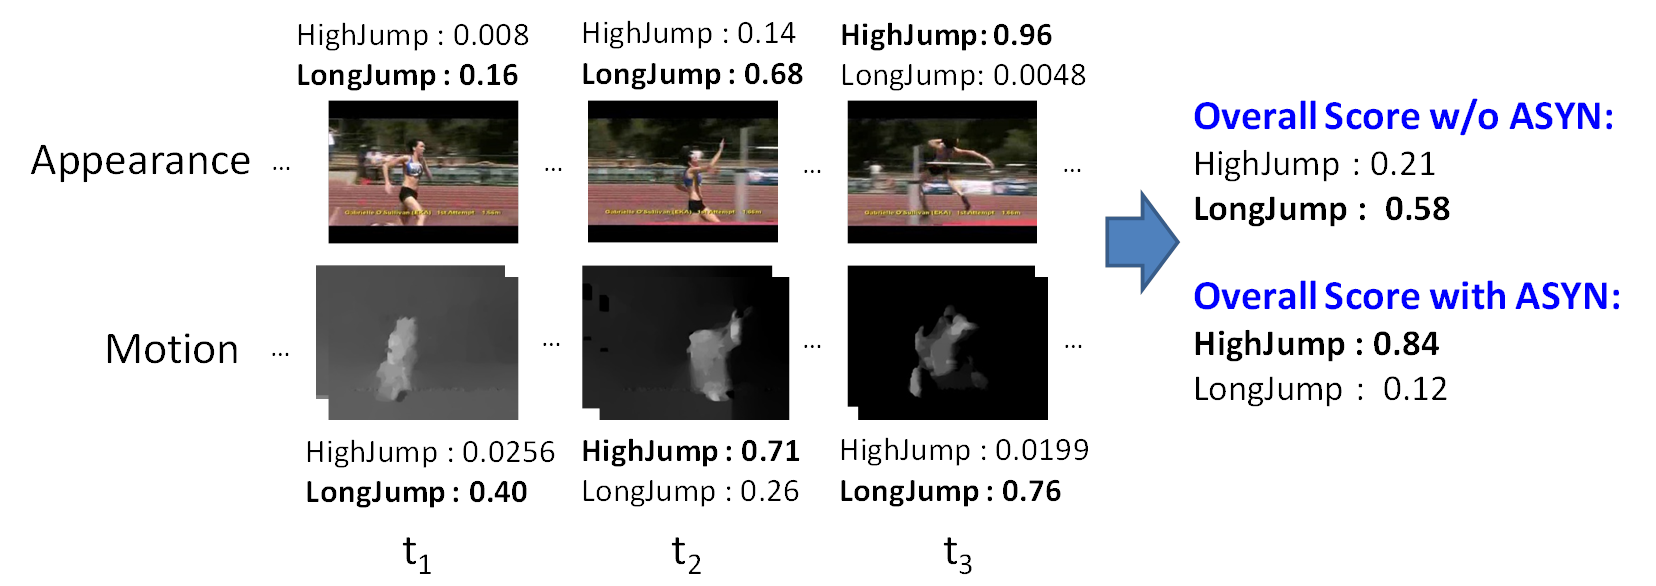
\includegraphics[width=0.47\textwidth,height=0.18\textwidth]{./figures1/exp.png}
  \caption{An example of the effect of the asynchronous fusion network: since two streams create high prediction scores for the ground-truth class ``Highjump" at different time points, the recognition result will be easily confused if not considering the stream-wise asynchronous pattern.} %(Note that the structure can also be used to fuse one frame input and multiple optical flow stack inputs. Best viewed in color)}
    \label{fig:exp}
\end{figure}




\subsection{Comparison with the state-of-the-art}

Table~\ref{tab:cmcTable3} compares our approach (\emph{CO2FI+ASYN}) with the state-of-the-art methods. Since many works reported results by performing a late fusion with hand-crafted IDT features~\cite{iDT}, we also show fusion result of our approach (\emph{CO2FI+ASYN+IDT}}). Note that in this experiment, we adopt three training/testing splits on both datasets in order to have a fair comparison with other methods.

%\cite{transform,TDDIDT,DIN}

%In Table~\ref{tab:cmcTable3}, \emph{CO2FI+ASYN} refers to the complete version of our approach where the coarse-to-fine and asynchronous fusion networks are integrated into the same framework. Since many works also reported results by performing a late fusion with hand-crafted IDT features, we also show fusion result of our approach (\emph{CO2FI+ASYN+IDT}}). %In order to further show the effectiveness of our approach, we also include the results where a roughly trained CNN\_M\_$2048$ ConvNet is used to form action class groups in the integrated framework \emph{CO2FI (rough)+ASYN}. Moreover, since many works also reported results by performing a late fusion with hand-crafted IDT features, we also show fusion result of our approach (\emph{CO2FI+ASYN+IDT}}).
%performing late fusion with hand-crafted IDT features can obtain a higher recognition result~\ref{tab:cmcTable2}, we also show the fused results between our approach and IDT in Table~\ref{tab:cmcTable3} (\emph{CO2FI+ASYN+IDT}}).

From Table~\ref{tab:cmcTable3}, we can see that our approach has better performances than most of the state-of-the-art methods. Specifically, when comparing with the most recent works using ResNet (\emph{ST-ResNet}) or introducing an additional information stream (\emph{ST-VLMPF}), our approach can also obtain similar or better results. This demonstrates the effectiveness of our proposed approach. Note that comparing with \emph{ST-ResNet} and \emph{ST-VLMPF}, we use a relatively short ConvNet (VGG-$16$) and do not introduce additional information streams. It is expected that the performances of our approach can be further improved if using deeper ConvNets such as ResNet or including more information streams. Moreover, our approach fused with IDT (\emph{CO2FI+ASYN+IDT}) also performs better than other IDT-fused methods. This furhter indicates the robustness of our approach in improving performances.

% or combining with other strategies such as feature encoding~\cite{LSTMSRC} \& spatial-temporal attention part selection~\cite{LSTMSRC}.

%Moreover, \emph{CO2FI (rough)+ASYN} method also achieves performance. This further demonstrates the importance of action class granularities, where action classes formed by a roughly trained model is already able to bring significant improvements.


\begin{table}
\centering
%\renewcommand\arraystretch{1.0}
\caption{Comparison of different methods (3 splits) %(note: the \emph{appearance} results of \emph{ASYN-Fusion} refer to the results by fusing one appearance input feature with multiple motion input features)
}\label{tab:cmcTable3}
\scriptsize{
%\label{table2}
\begin{tabular}{|p{5.3cm}|c|*{5}{c|}c}
\hline
\textbf{Methods}& UCF101& HMDB51 \\
\hline
C3D (3 nets) [Tran \emph{et al.} 2015]&  85.2\%& -- \\%\\
AdaScan [Kar \emph{et al.} 2017] &  89.4\%& 54.9\% \\%\\
TDD+FV [Wang \emph{et al.} 2015]&  90.3\%& 63.2\% \\%\\
%LTC [Varol \emph{et al.} 2016]&  91.7\%& 64.8\%\\
GRP [Cherian \emph{et al.} 2017]&  91.9\%& 65.4\%\\
Three-stream sDTD [Shi \emph{et al.} 2017]&  92.2\%& 65.2\%\\
Transformations [Wang \emph{et al.} 2016] &  92.4\%& 62.0\%\\  % 92.4% 62.0%
Two-Stream Fusion [Feichtenhofer \emph{et al.} 2016]&  92.5\%& 65.4\%\\
KVMF [Zhu \emph{et al.} 2016]&  93.1\%& 63.3\%\\
ST-ResNet [Feichtenhofer \emph{et al.} 2016]&  93.4\%& 66.4\%\\
L$^2$STM [Sun \emph{et al.} 2017]&  93.6\%& 66.2\%\\
ST-VLMPF [Duta \emph{et al.} 2017]&  93.6\%& {\bf 69.5}\%\\
TSN (2 modelities) [Wang \emph{et al.} 2016b] &  94.0\%& 68.5\%\\
%TSN (3 modelities) [Wang \emph{et al.} 2016b] &  {94.2}\%& 69.4\%\\
%ST-Multiplier [Feichtenhofer \emph{et al.} 2017]&  94.2\%& 68.9\%\\
{\bf CO2FI + ASYN}& {\bf 94.3\%}& {69.0\%}  \\
\hline
%CO2FI (rough)+ASYN & 93.2\%& 68.3\%  \\
Dynamic Image Networks + IDT [Bilen \emph{et al.} 2016] &  89.1\%& 65.2\% \\%\\
AdaScan + IDT [Kar \emph{et al.} 2017] &  91.3\%& 61.0\% \\%\\
TDD + IDT [Wang \emph{et al.} 2015]&  91.5\%& 65.9\%\\
GRP + IDT [Cherian \emph{et al.} 2017]&  92.3\%& 67.0\%\\
%Two-Stream Fusion+IDT [Feichtenhofer \emph{et al.} 2016]&  93.5\%& 69.2\%\\
ST-ResNet + IDT [Feichtenhofer \emph{et al.} 2016]&  94.6\%& 70.3\%\\
%ST-Multiplier+IDT [Feichtenhofer \emph{et al.} 2017]&  94.9\%& 72.2\%\\
{\bf CO2FI + ASYN + IDT}& {\bf 95.2\%}& {\bf 72.6\%}  \\
\hline
\end{tabular}}
\end{table}



%Note that we use a relatively small ConvNet (VGG-$16$) to extract features in our approach. It is expected that the performances of our approach can be further improved if using larger ConvNets such as ResNet~\cite{LSTMSRC}, or combining with other modules such as the asynchronous fusion network (as shown in Table~\ref{tab:cmcTable1}).


\section{Conclusion\label{section:conclusion}}


This paper presents a novel framework for action recognition. Our framework consists of two key ingredients: 1) a coarse-to-fine network, which extracts and integrates deep features from multiple action class
granularities to obtain a more precise feature representation for actions; 2) an asynchronous fusion network which integrates stream-wise features at different time points
for better leveraging the information in multiple streams.
Experimental results show that our approach achieves the state-of-the-art performance.

%{\color{red}C3D~\cite{c3d}, TDD~\cite{TDDIDT}, LTC~\cite{LTC}, Transformations~\cite{transform}, KVMF~\cite{KVMF}, ST-ResNet~\cite{nips}, TSN~\cite{TSN}, and Dynamic Image Networks~\cite{DIN}.}


%References and End of Paper
%These lines must be placed at the end of your paper
\bibliography{egbib}
\bibliographystyle{aaai}
\end{document}

